\chapter{刚体的转动}
\section{刚体转动的描述}
\section{惯量张量}
记单位张量为\(\vb{e}\)（为了与惯量张量区分，等价于其他章节的\(\vb{I}\)），定义刚体相对质心的惯量张量为：
\begin{align*}
	\vb{I} = \int \rho(\vb{r}) (r^2 \vb{e} - \vb{r} \vb{r}) \, \dd V.
\end{align*}
其中\(\vb{r}\)是体积元\(\dd V\)相对于质心的位矢.

对于相对于质心的位矢为\(\vb{a}\)的点\(P\)，定义刚体相对\(P\)点的惯量张量为：
\begin{align*}
	\vb{I}_P = \int \rho(\vb{r}) \left((r + a)^2 \vb{e} - (\vb{r} + \vb{a})(\vb{r} + \vb{a})\right) \, \dd V = \vb{I} + M (a^2 \vb{e} - \vb{a} \vb{a}),
\end{align*}
其中\(M = \int \rho(\vb{r}) \, \dd V\)是刚体的总质量.

当刚体以质心速度\(\vb{v}_C\)平动，以相对质心的角速度\(\vb{\omega}\)转动时，总动能为
\begin{align*}
	T = \frac{1}{2} \int \rho(\vb{r}) |\vb{v}_C + \vb{\omega} \times \vb{r}|^2 \, \dd V = \frac{1}{2} M v_c^2 + \frac{1}{2} \vb{I} : \vb{\omega} \vb{\omega}.
\end{align*}

相对质心的角动量为
\begin{align*}
	\vb{L}_c = \int \rho(\vb{r}) \vb{r} \times (\vb{\omega} \times \vb{r}) \, \dd V = \vb{I} \cdot \vb{\omega}.
\end{align*}

定义刚体相对穿过质心且单位方向为\(\uv{n}\)的转轴的转动惯量为：
\begin{align*}
	I(\uv{n}) = \int \rho(\vb{r}) |\uv{n} \times \vb{r}|^2 \, \dd V = \vb{I} : \uv{n} \uv{n}.
\end{align*}

对于相对于质心的位矢为\(\vb{a}\)的点\(P\)，定义刚体相对穿过\(P\)且单位方向为\(\uv{n}\)的转轴的转动惯量为：
\begin{align*}
	I_P(\uv{n}) = \int \rho(\vb{r}) |\uv{n} \times (\vb{r} + \vb{a})|^2 \, \dd V = \vb{I}_P : \uv{n} \uv{n} = I(\uv{n}) + M |\vb{a} \times \uv{n}|^2.
\end{align*}

\section{欧拉角}
选取随刚体一起平动的\(x\)-\(y\)-\(z\)坐标系，和随刚体一起转动的\(x_1\)-\(x_2\)-\(x_3\)坐标系，两坐标系原点均为\(O\).

如图\ref{欧拉角示意图}，定义欧拉角\(\theta\)，\(\varphi\)，\(\psi\)，使得\(x_1\)-\(x_2\)-\(x_3\)坐标系可以由\(x\)-\(y\)-\(z\)坐标系通过以下操作得到：
1. \(x\)-\(y\)绕\(z\)轴旋转\(\varphi\)得到\(x'\)，\(y'\)，将\(z\)更名为\(z'\)；
2. \(y'\)-\(z'\)绕\(x'\)轴旋转\(\theta\)得到\(y''\)，\(z''\)，将\(x'\)更名为\(x''\)；
3. \(x''\)-\(y''\)绕\(z''\)轴旋转\(\psi\)得到\(x'''\)，\(y'''\)，将\(z''\)更名为\(z'''\)；
\(x'''\)-\(y'''\)-\(z'''\)坐标系即为\(x_1\)-\(x_2\)-\(x_3\)坐标系.
\begin{figure}[htbp]
	\centering
	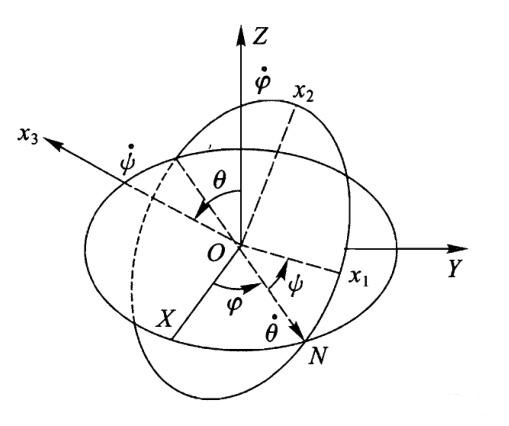
\includegraphics[width=0.3\textwidth]{rigid_body_fig/euler_angles_schematic_diagram.jpg}
	\caption{欧拉角示意图}
	\label{欧拉角示意图}
\end{figure}

用矩阵表示，这三次旋转的变换矩阵即为：
\begin{align*}
	R_1 = \begin{pmatrix}
		\cos \varphi  & \sin \varphi & 0 \\
		-\sin \varphi & \cos \varphi & 0 \\
		0             & 0            & 1
	\end{pmatrix}, \quad
	R_2 = \begin{pmatrix}
		1 & 0            & 0           \\
		0 & \cos \theta  & \sin \theta \\
		0 & -\sin \theta & \cos \theta
	\end{pmatrix}, \quad
	R_3 = \begin{pmatrix}
		\cos \psi  & \sin \psi & 0 \\
		-\sin \psi & \cos \psi & 0 \\
		0          & 0         & 1
	\end{pmatrix};
\end{align*}
\begin{align*}
	R = R_3 R_2 R_1 = \begin{pmatrix}
		\cos \psi \cos \varphi - \sin \psi \sin \varphi \cos \theta  & \sin \varphi \cos \psi + \cos \theta \cos \varphi \sin \psi  & \sin \theta \sin \psi \\
		-\sin \psi \cos \varphi - \cos \psi \sin \varphi \cos \theta & -\sin \varphi \sin \psi + \cos \theta \cos \varphi \cos \psi & \sin \theta \cos \psi \\
		\sin \theta \sin \varphi                                     & -\sin \theta \cos \varphi                                    & \cos \theta
	\end{pmatrix};
\end{align*}
\begin{align*}
	\begin{pmatrix}
		\uv{x}_1 \\
		\uv{x}_2 \\
		\uv{x}_3
	\end{pmatrix} = R \begin{pmatrix}
		\uv{x} \\
		\uv{y} \\
		\uv{z}
	\end{pmatrix}, \quad R^{-1} = R^\top.
\end{align*}

易知，刚体的角速度为
\begin{align*}
	\vb{\omega} = \dot{\theta}\, \uv{ON} + \dot{\varphi} \uv{z} + \dot{\psi} \uv{x_3},
\end{align*}
其中
\begin{align*}
	\uv{ON} = \uv{x} \cos \varphi + \uv{y} \sin \varphi = \uv{x}_1 \cos \psi - \uv{x}_2 \sin \psi.
\end{align*}

代入基矢变换关系得：
\begin{align*}
	\vb{\omega} & = (\dot{\theta} \cos \varphi + \dot{\psi} \sin \theta \sin \varphi) \uv{x} + (\dot{\theta} \sin \varphi - \dot{\psi} \sin \theta \cos \varphi) \uv{y} + (\dot{\varphi} + \dot{\psi} \cos \theta) \uv{z}=\omega_x \uv{x}+\omega_y \uv{y}+\omega_z \uv{z}        \\
	\vb{\omega} & = (\dot{\varphi} \sin \theta \sin \psi + \dot{\theta} \cos \psi) \uv{x}_1 + (\dot{\varphi} \sin \theta \cos \psi - \dot{\theta} \sin \psi) \uv{x}_2 + (\dot{\varphi} \cos \theta + \dot{\psi}) \uv{x}_3=\omega_1 \uv{x}_1+\omega_2 \uv{x}_2+\omega_3 \uv{x}_3.
\end{align*}

设\(x_1\)，\(x_2\)，\(x_3\)为刚体相对\(O\)的惯量张量\(\vb{I}\)的三个主轴：
\begin{align*}
	\vb{I} = I_1 \uv{x}_1 \uv{x}_1 + I_2 \uv{x}_2 \uv{x}_2 + I_3 \uv{x}_3 \uv{x}_3.
\end{align*}

则刚体相对\(O\)的动能为：
\begin{align*}
	T & = \frac{1}{2} \int \rho(\vb{r}) |\vb{\omega} \times \vb{r}|^2 \, \dd V = \frac{1}{2} \vb{I} : \vb{\omega} \vb{\omega} = \frac{1}{2} I_1 \omega_1^2 + \frac{1}{2} I_2 \omega_2^2 + \frac{1}{2} I_3 \omega_3^2\notag           \\
	  & = \frac{1}{2} I_1 (\dot{\varphi}^2 \sin^2 \theta + \dot{\theta}^2) + \frac{1}{2} I_3 (\dot{\varphi} \cos \theta + \dot{\psi})^2 + \frac{1}{2} (I_2 - I_1) (\dot{\varphi} \cos \psi \sin \theta - \dot{\theta} \sin \psi)^2.
\end{align*}

刚体相对\(O\)点的角动量为：
\begin{align*}
	\vb{L}_{O} & = I_1 \omega_1 \uv{x}_1 + I_2 \omega_2 \uv{x}_2 + I_3 \omega_3 \uv{x}_3\notag                                                                                                                                        \\
	           & = I_1 (\dot{\varphi} \sin \theta \sin \psi + \dot{\theta} \cos \psi) \uv{x}_1 + I_2 (\dot{\varphi} \sin \theta \cos \psi - \dot{\theta} \sin \psi) \uv{x}_2 + I_3 (\dot{\varphi} \cos \theta + \dot{\psi}) \uv{x}_3.
\end{align*}
\section{刚体的自由转动}
记刚体总质量为\(M\)，记关于质心的转动惯量主轴为1，2，3轴，相应的转动惯量为\(I_1\)，\(I_2\)，\(I_3\).

记刚体所受合外力为\(\vb{F}\)、相对质心外力矩为\(\vb{\tau}\)，刚体质心速度为\(\vb{v}_c\)，刚体角速度为\(\vb{\omega}\)，则刚体运动方程为
\begin{align*}
	\vb{F} = M \frac{\dd \vb{v}_c}{\dd t}, \quad \vb{\tau} = \frac{\dd \vb{L}_c}{\dd t} = \left(\frac{\dd \vb{L}_c}{\dd t}\right)_c + \vb{\omega}\times\vb{L}_c,
\end{align*}
其中\(\vb{L}_c\)为刚体相对质心的角动量，下标\(c\)代表在随刚体转动的系中求导（该系中基矢\(\hat{\vb{x}_i}\)不动）.

由\(\vb{L}_c = I_1 \omega_1 \uv{x}_1 + I_2 \omega_2 \uv{x}_2 + I_3 \omega_3 \uv{x}_3\)，可以展开得欧拉方程：
\begin{align*}
	I_1 \dot{\omega}_1 + (I_3 - I_2)\omega_2\omega_3 & = \tau_1, \\
	I_2 \dot{\omega}_2 + (I_1 - I_3)\omega_3\omega_1 & = \tau_2, \\
	I_3 \dot{\omega}_3 + (I_2 - I_1)\omega_1\omega_2 & = \tau_3.
\end{align*}

刚体做自由转动指\(\vb{\tau} = \vb{0}\)，此时，由上式易知，转动动能守恒，角动量守恒：
\begin{align*}
	\vb{L} = \vb{L}_c = I_1 \omega_1 \uv{x}_1 + I_2 \omega_2 \uv{x}_2 + I_3 \omega_3 \uv{x}_3 = \text{const},
\end{align*}
\begin{align*}
	E = \frac{1}{2}I_1\omega_1^2 + \frac{1}{2}I_2\omega_2^2 + \frac{1}{2}I_3\omega_3^2 = \text{const}.
\end{align*}

不妨假设\(I_3 \geq I_2 \geq I_1\)（进而下式\(2EI_1 \leq L^2 \leq 2EI_3\)），选取如下三个独立方程描述转动：
\begin{align*}
	L^2 = I_1^2\omega_1^2 + I_2^2\omega_2^2 + I_3^2\omega_3^2,
\end{align*}
\begin{align*}
	2E = I_1\omega_1^2 + I_2\omega_2^2 + I_3\omega_3^2,
\end{align*}
\begin{align*}
	I_2 \dot{\omega}_2 + (I_1 - I_3)\omega_1\omega_3 = 0.
\end{align*}

给出
\begin{align*}
	\omega_1^2 &= \frac{1}{I_1(I_3-I_1)}\left[(2EI_3 - L^2) - I_2(I_3-I_2)\omega_2^2\right],\\
	\omega_3^2 &= \frac{1}{I_3(I_3-I_1)}\left[(L^2 - 2EI_1) - I_2(I_2-I_1)\omega_2^2\right].\\
	&\left(\frac{\dd \omega_2}{\dd t}\right)^2 = \frac{1}{I_2^2 I_1 I_3}\left[(2EI_3 - L^2) - I_2(I_3-I_2)\omega_2^2\right]\left[(L^2 - 2EI_1) - I_2(I_2-I_1)\omega_2^2\right].
\end{align*}

从演化方程可初步看出，\(\omega_2^2\)存在上限、下限为\(0\)，其将在上下限之间周期性演化.另外，\(L^2\)与\(2EI_2\)的大小关系也将影响解\(\omega_2(t)\)的数学形式.

由于地面系下\(\vb{L}\)是常矢量，不妨选取欧拉角中的\(z\)轴平行于\(\vb{L}\)，则：
\begin{align*}
	\vb{L}=L\,\uv{z}= I_1 \omega_1 \uv{x}_1 + I_2 \omega_2 \uv{x}_2 + I_3 \omega_3 \uv{x}_3 ,
\end{align*}
\begin{align*}
	I_1\omega_1 = L\sin\theta\sin\psi, \quad I_2\omega_2 = L\sin\theta\cos\psi, \quad I_3\omega_3 = L\cos\theta.
\end{align*}
得到欧拉角与角速度的关系为：
\begin{align*}
	\cos\theta = \frac{I_3\omega_3}{L}, \quad \tan\psi = \frac{I_1\omega_1}{I_2\omega_2},\quad \dot{\varphi} = \frac{\omega_1\sin\psi + \omega_2\cos\psi}{\sin\theta} = L \frac{I_1\omega_1^2 + I_2\omega_2^2}{I_1^2\omega_1^2 + I_2^2\omega_2^2}.
\end{align*}

下将演示，如何根据演化方程，通过椭圆函数形式给出\(\vb{\omega},\theta,\psi,\varphi\)与时间\(t\)的关系.

\textbf{情况一.  \(L^2 \leq 2EI_2\)}

定义参数
\begin{align*}
	k^2 = \frac{(I_3-I_2)(L^2-2EI_1)}{(I_2-I_1)(2EI_3-L^2)}, \quad 0 \leq k^2 < 1
\end{align*}
引入变量变换
\begin{align*}
	\tau = t\sqrt{\frac{(I_2-I_1)(2EI_3-L^2)}{I_1I_2I_3}}, \quad
	s = \omega_2\sqrt{\frac{I_2(I_2-I_1)}{L^2-2EI_1}}
\end{align*}
演化方程简化为
\begin{align*}
	\left(\frac{\dd s}{\dd \tau}\right)^2 = (1-s^2)(1-k^2s^2)
\end{align*}
取初值\(\omega_2(t=0)=0\)，解得
\begin{align*}
	s(\tau) = \sn(\tau,k)
\end{align*}
进而
\begin{align*}
	\omega_1      & = \sqrt{\frac{2EI_3-L^2}{I_1(I_3-I_1)}}\dn(\tau,k) ,\quad
	\omega_2=\sqrt{\frac{2EI_1-L^2}{I_2(I_2-I_1)}} \sn(\tau,k),\quad
	\omega_3 = \sqrt{\frac{L^2-2EI_1}{I_3(I_3-I_1)}}\cn(\tau,k),                                               \\
	\cos\theta    & = \sqrt{\frac{I_3(L^2-2EI_1)}{L^2(I_3-I_1)}}\cn(\tau,k),\quad
	\tan\psi = \sqrt{\frac{I_1(I_2-I_1)(2EI_3-L^2)}{I_2(I_3-I_1)(L^2-2EI_1)}}\frac{\dn(\tau,k)}{\sn(\tau,k)},  \\
	\dot{\varphi} & = L \frac{(2EI_3-L^2)+(L^2-2EI_1)\sn^2(\tau,k)}{I_1(2EI_3-L^2)+I_3(L^2-2EI_1)\sn^2(\tau,k)}.
\end{align*}

运动周期（同样也是\(\vb{\omega}\)的演化周期）为
\begin{align*}
	T = 4\sqrt{\frac{I_1I_2I_3}{(I_2-I_1)(2EI_3-L^2)}}\int_0^1\frac{\dd x}{\sqrt{(1-x^2)(1-k^2x^2)}}= 4\sqrt{\frac{I_1I_2I_3}{(I_2-I_1)(2EI_3-L^2)}}F(k)
\end{align*}

\textbf{情况二.  \(L^2 \geq 2EI_2\)}

定义参数
\begin{align*}
	k^2 = \frac{(I_2-I_1)(2EI_3-L^2)}{(I_3-I_2)(L^2-2EI_1)}, \quad 0 \leq k^2 < 1
\end{align*}
引入变量变换
\begin{align*}
	\tau = t\sqrt{\frac{(I_3-I_2)(L^2-2EI_1)}{I_1I_2I_3}}, \quad
	s = \omega_2\sqrt{\frac{I_2(I_3-I_2)}{2EI_3-L^2}}
\end{align*}
演化方程简化为
\begin{align*}
	\left(\frac{\dd s}{\dd \tau}\right)^2 = (1-s^2)(1-k^2s^2)
\end{align*}
取初值\(\omega_2(t=0)=0\)，解得
\begin{align*}
	s(\tau) = \sn(\tau,k)
\end{align*}
进而
\begin{align*}
	\omega_1      & = \sqrt{\frac{2EI_3-L^2}{I_1(I_3-I_1)}}\cn(\tau,k),\quad
	\omega_2=\sqrt{\frac{2EI_3-L^2}{I_2(I_3-I_2)}} \sn(\tau,k),\quad
	\omega_3 = \sqrt{\frac{L^2-2EI_1}{I_3(I_3-I_1)}}\dn(\tau,k),                                       \\
	\cos\theta    & = \sqrt{\frac{I_3(L^2-2EI_1)}{L^2(I_3-I_1)}}\dn(\tau,k) ,\quad
	\tan\psi = \sqrt{\frac{I_1(I_3-I_2)}{I_2(I_3-I_1)}}\frac{\cn(\tau,k)}{\sn(\tau,k)} ,               \\
	\dot{\varphi} & = \frac{(I_3-I_2)+(I_2-I_1)\sn^2(\tau,k)}{I_1(I_3-I_2)+I_3(I_2-I_1)\sn^2(\tau,k)}.
\end{align*}

运动周期为
\begin{align*}
	T = 4 \sqrt{\frac{I_1 I_2 I_3}{(I_3 - I_2)(L^2 - 2EI_1)}} \int_0^1 \frac{\dd x}{\sqrt{(1-x^2)(1-k^2 x^2)}}= 4 \sqrt{\frac{I_1 I_2 I_3}{(I_3 - I_2)(L^2 - 2EI_1)}} F(k)
\end{align*}

\textbf{情况三.  \(L^2 = 2EI_2\)}

对以上两种情况取极限即可
\begin{align*}
	\omega_1      & = \omega_0\sqrt{\frac{I_2(I_3-I_2)}{I_1(I_3-I_1)}}\sech(\Omega t) ,\quad
	\omega_2 = \omega_0\tanh(\Omega t) ,\quad
	\omega_3 = \omega_0\sqrt{\frac{I_2(I_2-I_1)}{I_3(I_3-I_1)}}\sech(\Omega t),                                              \\
	\cos\theta    & = \sqrt{\frac{I_3(I_2-I_1)}{I_2(I_3-I_1)}}\sech(\Omega t) ,\quad
	\tan\psi = \sqrt{\frac{I_1(I_3-I_2)}{I_2(I_3-I_1)}}\mathrm{csch}(\Omega t) ,                                             \\
	\dot{\varphi} & = \omega_0\frac{I_2(I_3-I_1)\sinh^2(\Omega t)+I_2(I_3-I_2)}{I_2(I_3-I_1)\sinh^2(\Omega t)+I_1(I_3-I_2)}.
\end{align*}
式中
\begin{align*}
	\omega_0 = \sqrt{\frac{2E}{I_2}} = \frac{L}{I_2},\quad \Omega = \omega_0\sqrt{\frac{(I_2-I_1)(I_3-I_2)}{I_1I_3}}
\end{align*}

当\(t \to \pm\infty\)时，角速度分别渐近于沿2轴方向的 \(\pm\omega_0\) 分量。这里的解是连接两个中间轴不稳定平衡点的异宿轨道；并非从精确初值 \((0,\omega_0,0)\) 出发后发生转移，因为该初值本身就是欧拉方程的不动点。在取上述解的 \(t=0\) 截面时，
\begin{align*}
	\omega_1= \omega_0 \sqrt{\frac{I_2(I_3-I_2)}{I_1(I_3-I_1)}} ,\quad
	\omega_2 = 0 ,\quad
	\omega_3 = \omega_0 \sqrt{\frac{I_2(I_2-I_1)}{I_3(I_3-I_1)}}.
\end{align*}

这表明在异宿轨道的有限时间截面，角速度同时具有1、3轴分量；在 \(t\to\pm\infty\) 时又渐近回到2轴，而不是长期停留在1、3轴上。

\textbf{情况四. 旋转对称刚体}

对于旋转对称刚体，取\(x_3\)为旋转对称轴，则有\(I_1 = I_2\)，同时取消\(I_1 \leq I_3\)的限制.

设\(t=0\)时刻初始条件为：
\begin{align*}
	\omega_1(0) = \omega_{10}, \quad \omega_2(0) = \omega_{20}, \quad \omega_3(0) = \omega_{30}
\end{align*}

则角动量、能量的表达式简化为
\begin{align*}
	L^2 = I_1^2(\omega_{10}^2 + \omega_{20}^2) + I_3^2\omega_{30}^2 ,\quad
	E = \frac{1}{2}I_1(\omega_{10}^2 + \omega_{20}^2) + \frac{1}{2}I_3\omega_{30}^2.
\end{align*}

以上各式简化为
\begin{align*}
	\omega_1 = \sqrt{\omega_{10}^2+\omega_{20}^2}\cos\left(\omega_{30}t\left|\frac{I_3-I_1}{I_1}\right|\right) ,\quad
	\omega_2 = \sqrt{\omega_{10}^2+\omega_{20}^2}\sin\left(\omega_{30}t\left|\frac{I_3-I_1}{I_1}\right|\right) ,\quad
	\omega_3 = \omega_{30} ,
\end{align*}
\begin{align*}
	\cos\theta = \frac{I_3\omega_{30}}{\sqrt{I_1^2(\omega_{10}^2+\omega_{20}^2)+I_3^2\omega_{30}^2}} ,\quad
	\psi = \frac{\pi}{2}-\omega_{30}t\left|\frac{I_3-I_1}{I_1}\right| ,\quad
	\varphi = \frac{\sqrt{I_1^2(\omega_{10}^2+\omega_{20}^2)+I_3^2\omega_{30}^2}}{I_1}t.
\end{align*}

运动周期为
\begin{align*}
	T = \frac{2\pi}{\omega_{30}\left|\frac{I_3-I_1}{I_1}\right|}.
\end{align*}

可见，旋转对称刚体将关于\(z\)轴做稳定进动，角速度矢量\(\vb{\omega}\)也将关于角动量矢量\(\vb{L}\)做稳定进动.

\begin{note}
	以上各情况可以根据如下解析延拓公式写成更为统一的形式
	\begin{align*}
		\sn(\tau,k)&=\frac{1}{k}\sn(k\tau,\frac{1}{k}),\quad \cn(\tau,k)=\dn(k\tau,\frac{1}{k}),\quad \dn(\tau,k)=\cn(k\tau,\frac{1}{k}).\\
		\sn(\tau,0)&=\sin\tau,\quad \cn(\tau,0)=\cos\tau,\quad \dn(\tau,0)=1.\\
		\sn(\tau,1)&=\tanh\tau,\quad \cn(\tau,1)=\dn(\tau,1)=\sech\tau.
	\end{align*}
\end{note}
\section{势场中的定点转动}
假设刚体表面 \(P\) 点被固定在地面上，\(P\) 相对于质心的位矢为 \(\vb{a}\)，则总动能为
\begin{align*}
	T= \frac{1}{2}\, M v_c^2 + \frac{1}{2}\, \vb{I} : \vb{\omega} \vb{\omega} = \frac{1}{2}\, M | \vb{\omega} \times \vb{a} |^2 + \frac{1}{2}\, \vb{I} : \vb{\omega} \vb{\omega} = \frac{1}{2}\, \vb{I}_P : \vb{\omega} \vb{\omega}.
\end{align*}

可以选用拉格朗日力学的方法，并取欧拉角 \(\theta\), \(\phi\), \(\psi\) 为三个独立的广义坐标，则总动能通常写作
\begin{align*}
	T = \frac{1}{2} I_{P1} (\dot{\phi}^2 \sin^2 \theta + \dot{\theta}^2) + \frac{1}{2} I_{P3} (\dot{\phi} \cos \theta + \dot{\psi})^2 + \frac{1}{2} (I_{P2} - I_{P1}) (\dot{\phi} \cos \psi \sin \theta - \dot{\theta} \sin \psi)^2,
\end{align*}
其中（记\(\vb{I}\)的三个主轴方向单位矢量为\(\uv{n}_1,\uv{n}_2,\uv{n}_3\)）
\begin{align*}
	I_{P1} = I_1 + M | \vb{a} \times \uv{n}_1 |^2,\quad I_{P2} = I_2 + M | \vb{a} \times \uv{n}_2 |^2, \quad I_{P3} =I_3 + M | \vb{a} \times \uv{n}_3 |^2.
\end{align*}

以旋转对称刚体在均匀重力场中的定点转动为例：
作为简化，假设刚体匀质，定点 \(P\) 恰位于旋转对称轴 \(x_3\) 上，距刚体质心为 \(a\)，刚体绝缘且均匀带有电荷量 \(Q\)，空间中存在与均匀重力场方向相反的匀强磁场 \(\vb{B}\)，刚体关于过 \(P\) 且平行于旋转对称轴的轴转动惯量为 \(I_3\)，关于过 \(P\) 且垂直于旋转对称轴的轴转动惯量为 \(I_1\)（简洁起见，省略了下标\(P\)），重力加速度为 \(g\).

令竖直向上为 \(z\) 轴正方向，采用拉格朗日力学的方法，并取欧拉角 \(\theta\), \(\phi\), \(\psi\) 为三个独立的广义坐标;
\begin{figure}[htbp]
	\centering
	
\includegraphics[width=0.4\textwidth]{rigid_body_fig/fixed_point_rigid_body_rotation_example_schematic_diagram.png}
	\caption{刚体定点转动例题示意图}
	\label{刚体定点转动例题示意图}
\end{figure}

记刚体的势能为\(V\)，空间磁矢势为\(\vb{A}\)，则刚体的拉格朗日量为：
\begin{align*}
	\mathcal{L} = T - V + \int \vb{A} \cdot \vb{v} \, \dd q = T - V + \int \left( \frac{1}{2} \vb{B} \times \vb{r} \right) \cdot \vb{v} \, \dd q = T - V + \vb{\Omega} \cdot \vb{L}.
\end{align*}
其中
\begin{align*}
	\vb{\Omega} = \frac{Q \vb{B}}{2 M} = \frac{Q B}{2 M} \uv{z}, \quad
	\vb{A} = \frac{1}{2} \vb{B} \times \vb{r} .
\end{align*}

根据之前部分的讨论
\begin{align*}
	\uv{z} = \sin \psi \sin \theta \uv{x}_1 + \sin \theta \cos \psi \uv{x}_2 + \cos \theta \uv{x}_3,
\end{align*}
\begin{align*}
	\vb{L} = I_1 (\dot{\phi} \sin \theta \sin \psi + \dot{\theta} \cos \psi) \uv{x}_1 + I_1 (\dot{\phi} \sin \theta \cos \psi - \dot{\theta} \sin \psi) \uv{x}_2  + I_3 (\dot{\phi} \cos \theta + \dot{\psi}) \uv{x}_3.
\end{align*}
又刚体的动能、势能为
\begin{align*}
	T = \frac{1}{2} I_1 (\dot{\theta}^2 + \dot{\phi}^2 \sin^2 \theta) + \frac{1}{2} I_3 (\dot{\psi} + \dot{\phi} \cos \theta)^2,\quad V = M g a \cos \theta.
\end{align*}
代入得
\begin{align*}
	\mathcal{L} = \Omega \left( I_1 \dot{\phi} \sin^2 \theta + I_3 (\dot{\phi} \cos \theta + \dot{\psi}) \cos \theta \right) + \frac{1}{2} I_1 (\dot{\theta}^2 + \dot{\phi}^2 \sin^2 \theta)  + \frac{1}{2} I_3 (\dot{\psi} + \dot{\phi} \cos \theta)^2 - M g a \cos \theta.
\end{align*}
进而，系统的广义动量为
\begin{align*}
	p_\theta & = \frac{\partial \mathcal{L}}{\partial \dot{\theta}} = I_1 \dot{\theta}, \quad p_\psi = \frac{\partial \mathcal{L}}{\partial \dot{\psi}} = I_3 (\dot{\psi} + (\dot{\phi} + \Omega) \cos \theta), \\
	p_\phi   & = \frac{\partial \mathcal{L}}{\partial \dot{\phi}} = p_\psi \cos \theta + I_1 (\dot{\phi} + \Omega) \sin^2 \theta.
\end{align*}
哈密顿量为
\begin{align*}
	\mathcal{H} =\displaystyle\sum_i p_i q_i-\mathcal{L}= T + V = \frac{p_\psi^2}{2 I_3} - \Omega p_\phi + \frac{p_\theta^2}{2 I_1} + \frac{(p_\phi - p_\psi \cos \theta)^2}{2 I_1 \sin^2 \theta} + \frac{1}{2} \Omega^2 (I_1 \sin^2 \theta + I_3 \cos^2 \theta) + M g a \cos \theta.
\end{align*}

由哈密顿方程得：\(p_\psi\) 守恒，\(p_\phi\) 守恒，以及
\begin{align*}
	\dot{p}_\theta = -\frac{\partial \mathcal{H}}{\partial \theta}\quad\implies\quad
	I_1 \ddot{\theta} = M g a \sin \theta + \Omega^2 (I_3 - I_1) \sin \theta \cos \theta - \frac{(p_\phi - p_\psi \cos \theta)(p_\psi - p_\phi \cos \theta)}{I_1 \sin^3 \theta}.
\end{align*}

给出，稳定运动下，\(\ddot{\theta} (\theta = \theta_0, \dot{\phi} = \dot{\phi}_0) = 0\)，有
\begin{align*}
	\dot{\psi}_0 & = \frac{M g a}{I_3 (\dot{\phi}_0 + \Omega)} - \frac{(\dot{\phi}_0 + \Omega)^2 - \Omega^2}{I_3 (\dot{\phi}_0 + \Omega)} (I_3 - I_1) \cos \theta_0.                                                        \\
	p_{\phi}     & = \frac{I_3 \Omega^2}{\dot{\phi}_0 + \Omega} \cos^2 \theta_0 + \frac{Mga \cos \theta_0}{\dot{\phi}_0 + \Omega} + I_1 \frac{(\dot{\phi}_0 + \Omega)^2 - \Omega^2 \cos^2 \theta_0}{\Omega + \dot{\phi}_0}, \\
	p_{\psi}     & = \frac{I_3 \Omega^2}{\dot{\phi}_0 + \Omega} \cos \theta_0 + \frac{Mga}{\dot{\phi}_0 + \Omega} + I_1 \cos \theta_0 \frac{(\dot{\phi}_0 + \Omega)^2 - \Omega^2}{\Omega + \dot{\phi}_0}.
\end{align*}

在稳态附近展开运动方程，并保留至最低阶项，得
\begin{align*}
	\ddot{\theta} =\omega_p^2 (-\theta + \theta_0).
\end{align*}
其中微扰角频率为
\begin{align*}
	\omega_p & =\left[ \left( \frac{M g a}{I_1 (\dot{\phi}_0 + \Omega)} \right)^2 - \frac{2 M g a}{I_1} \cos \theta_0 + (\dot{\phi}_0 + \Omega)^2 \right. + (1 - 3 \cos^2 \theta_0) \left( \frac{I_3}{I_1} - 1 \right) \Omega^2 \\&\qquad+ \frac{\Omega^4 \cos^2 \theta_0}{(\dot{\phi}_0 + \Omega)^2} \left( \frac{I_3}{I_1} - 1 \right)^2 + \left. \frac{2 M g a \Omega^2 \cos \theta_0}{I_1 (\dot{\phi}_0 + \Omega)^2} \left( \frac{I_3}{I_1} - 1 \right) \right]^{\frac{1}{2}}
\end{align*}

引入 \(\alpha = M g a/I_1 \Omega^2\), \(\beta = \dot{\phi}_0/\Omega\), \(\gamma = I_3/I_1\)，化简得

\begin{align*}
	\dot{\psi}_0 = \Omega \left( \frac{\alpha}{\gamma (1 + \beta)} - \frac{(1 + \beta)^2 - 1}{\gamma (1 + \beta)} (\gamma - 1) \cos \theta_0 \right),
\end{align*}
\begin{align*}
	\omega_p = \Omega \left[ \frac{\alpha^2}{(1 + \beta)^2} - 2 \alpha \cos \theta_0 + (1 + \beta)^2 \right.+ (-1 + \gamma) \left( \frac{2 \alpha \cos \theta_0}{(1 + \beta)^2} - 3 \cos^2 \theta_0 + 1 \right) + \left. \frac{\cos^2 \theta_0}{(1 + \beta)^2} (-1 + \gamma)^2 \right]^{1/2}.
\end{align*}

\begin{exbox}
	若刚体为旋转对称心形，其截面的边界为 \(r (\theta) = R (1 - \cos \theta)\), \(P\) 恰位于 \(\theta = \pi\) 处，
	则
	\begin{align*}
		a = \frac{6}{5} R, \quad M = \frac{8 \pi}{3} \rho R^3, \quad I_1 = \frac{192}{35} \pi \rho R^5, \quad I_3 = \frac{64}{35} \pi \rho R^5,\quad
		\alpha = \frac{M g a}{I_1\Omega^2}
		= \frac{35}{72}\frac{a}{R}\frac{g}{R\Omega^2}
		= \frac{7}{10}, \quad \gamma = \frac{1}{3}.
	\end{align*}

	给定数值 \(\beta = 7.684,\, \dfrac{g}{R\Omega^2}=1.2,\, \theta_0=1.47\,\mathrm{rad}\)，可计算得
	\begin{align*}
		\frac{\dot{\psi}_0}{\Omega} & = 1.966, \quad \frac{\omega_p}{\Omega} = 8.639.
	\end{align*}
\end{exbox}

\begin{exbox}
	只考虑重力场，无电学作用(\(\Omega=0\))，给出
	\begin{align*}
		\dot{\psi}_0 = \frac{M g a}{I_3 \dot{\phi}_0} - \frac{I_3-I_1}{I_3}\dot{\phi}_0\cos \theta_0.\quad
		\omega_p=\sqrt{\dot{\phi}_0^2-\frac{2Mga}{I_1}\cos\theta_0+\left(\frac{Mga}{I_1\dot{\phi}_0}\right)^2}.
	\end{align*}
\end{exbox}

\begin{note}
	该问题也可以用传统的矢量方法解决，物理上更直观，但计算较繁琐.

	记质心相对参考点位矢为 \(\vb{r}_c\,\)，刚体上某一点相对质心的位矢为 \(\vb{r}'\)，刚体的质量密度为 \(\rho(\vb{r}')\)，相对质心的惯量张量为 \(\vb{I}= \int \rho(\vb{r}') \left( r'^2 \vb{e} - \vb{r}' \vb{r}' \right) \dd \vb{r}'\)，
	总质量为 \(M = \int \rho(\vb{r}') \dd \vb{r}'\).电荷密度为 \(\rho_e(\vb{r}')\)，总电荷量为 \(Q = \int \rho_e(\vb{r}') \dd \vb{r}'\).假设其荷质比为常数 \(Q/M\)，即 \(\rho_e(\vb{r}) = Q \,\rho(\vb{r})/M\).
	空间中存在匀强磁场 \(\vb{B}\)，记 \(\vb{\Omega} = Q\vb{B}/2M\).

	当刚体质心以速度 \(\vb{v}_c\) 运动、刚体相对质心以角速度 \(\vb{\omega}\) 转动时，刚体上 \(\vb{r}_c + \vb{r}'\) 处的质点的速度为 \(\vb{v}(\vb{r}') = \vb{v}_c + \vb{\omega} \times \vb{r}'\)，
	其中用到\(\dd \vb{r}'/\dd t = \vb{\omega} \times \vb{r}'\).

	进而，刚体所受电磁合外力为
	\begin{align*}
		\vb{F}_{\text{em}} = \int \rho_e(\vb{r}') \vb{v}(\vb{r}') \times \vb{B} \dd \vb{r}' = Q \vb{v}_c \times \vb{B},
	\end{align*}

	电磁合外力矩为
	\begin{align*}
		\vb{\tau}_{\text{em}} & = \int \rho_e(\vb{r}') (\vb{r}_c + \vb{r}') \times (\vb{v}(\vb{r}') \times \vb{B}) \dd \vb{r}' = Q \vb{r}_c \times (\vb{v}_c \times \vb{B}) + \int 2 \rho(\vb{r}') \vb{r}' \times [(\vb{\omega} \times \vb{r}') \times \vb{\Omega}]                                           \\
		                      & = Q \vb{r}_c \times (\vb{v}_c \times \vb{B}) + \int \rho(\vb{r}') \left[ \frac{\dd}{\dd t} \left( \vb{r}' (\vb{r}' \cdot \vb{\Omega}) - r'^2 \vb{\Omega} \right) + \vb{\Omega} \times \left( \vb{r}' (\vb{r}' \cdot \vb{\omega}) - r'^2 \vb{\omega} \right) \right] \dd \vb{r}' \\
		                      & = Q \vb{r}_c \times (\vb{v}_c \times \vb{B}) - \frac{\dd}{\dd t} (\vb{I} \cdot \vb{\Omega}) - \vb{\Omega} \times (\vb{I} \cdot \vb{\omega})
	\end{align*}

	应用于以上情形，也可得到正确结果.
\end{note}
